\subsubsection{Weather shielding}
The custom rotator is designed to operate in outdoor environment for long duration. To avoid damage from sun light exposure and humidity, a dedicated shielding is designed for mechanical and electronics parts. The architecture of shielding is based on consideration that shielding should not hinder the mechanical movements of any part. 
\subsubsection*{Weather shielding design methodology}
The design of shielding is optimised to provide protection to the critical parts. Materials, manufacturing process and parts are from off shelf technologies and easy to manufacture. Manufacturing materials are aluminium sheet and 3D printed abs plastic. Following figure shows various components of shielding marked in green and white colour.     
\begin{figure}[H]
	\centering
	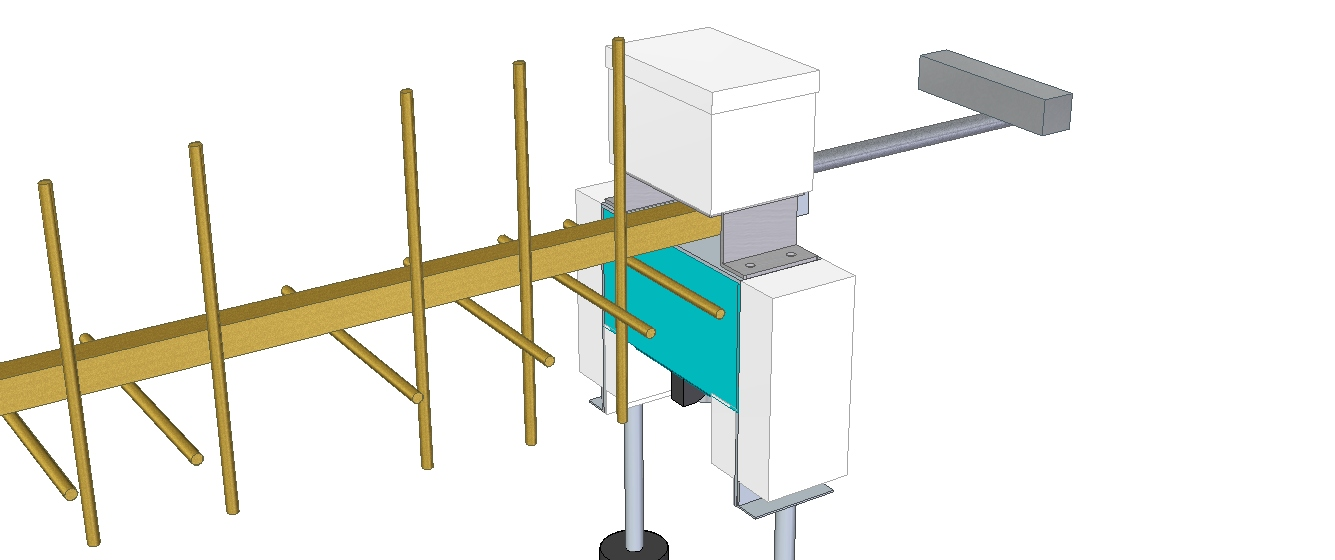
\includegraphics[width=\linewidth]{../art/overing.jpg}
	\caption{Rotator with Shielding}
\end{figure}

The differential shielding (green color) is responsible to provide free movement to the rotator. The design is inspired from the military vehicle design. In this approach, a grove is provided for movement of shaft and this whole structure is covered with a flexible sheet (black in colour) to provide movement capability and seal. 

\subsubsection*{Belt covering}
Belt covering is provided by 3D printed abs plastic structure and mounted by nuts and bolts on main frame. It provides easy access for repair and routine checks. Following image shows the design and the way it is going to cover the belt and pulley. The remaining top of the belt will be covered in differential shielding.     
\begin{figure}[H]
	\centering
	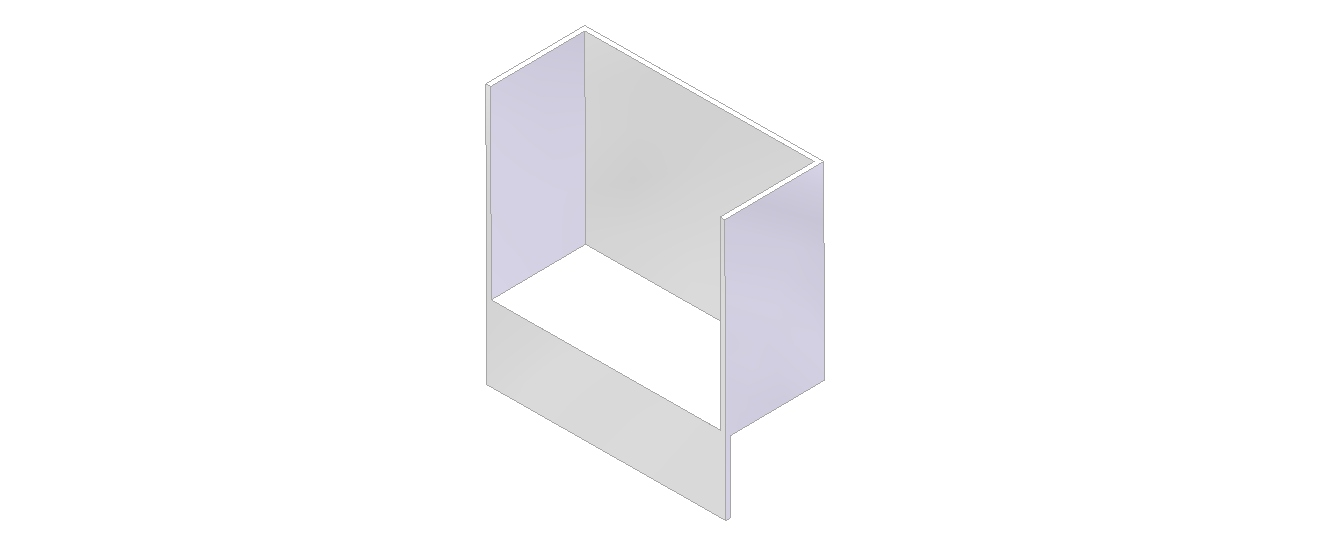
\includegraphics[width=0.7\linewidth]{../art/belt cover.jpg}
	\caption{Belt Covering}
\end{figure}

\subsubsection*{Motor covering}
Motor covering is provided by 3D printed abs plastic structure and mounted by nuts and bolts on main frame. It provides easy access for repair and routine checks. Following image shows the design and the way it is going to cover motor.     
\begin{figure}[H]
	\centering
	
\includegraphics[width=0.8\linewidth]{../art/motor cover.jpg}
	\caption{Motor Covering}
\end{figure}

\subsubsection*{Electronics Covering}
Electronics box is designed by using 3D printed abs plastic structure and mounted by nuts and bolts on main frame. It provides easy access for repair and routine checks. It is simple cuboid box with top cover lid. It is designed to provide required volume for controllers, receiver and wiring.    
\begin{figure}[H]
	\centering
	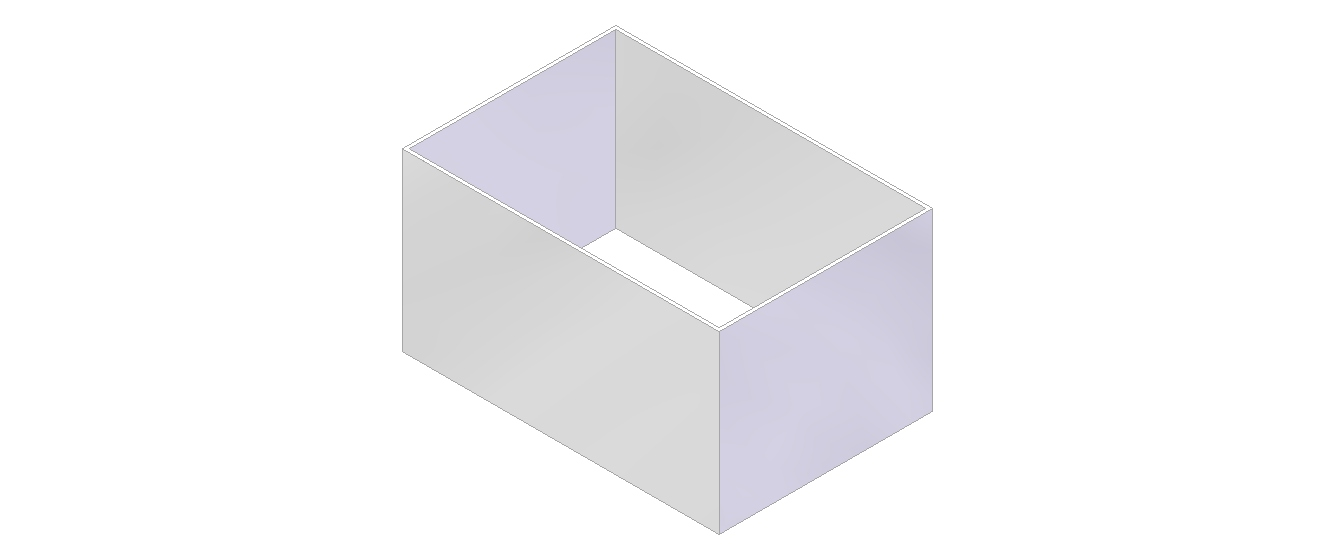
\includegraphics[width=0.7\linewidth]{../art/elec.jpg}
	\caption{Electronics Covering}
\end{figure}

